\documentclass[11pt,a4paper]{moderncv}
\moderncvtheme[blue]{banking}                
\usepackage[utf8]{inputenc}
\usepackage[top=1.3cm, bottom=1.3cm, left=2cm, right=2cm]{geometry}
\usepackage[english]{babel}
\setlength{\hintscolumnwidth}{2.9cm} % width of the left column (dates)
%\setlength{\makecvtitlenamewidth}{20cm}
%\setlength{\maketitlewidth}{\textwidth}
%\setlength{\maketitleboxwidth}{\textwidth}
%\setlength{\maketitlewidth}{\textwidth}
%\setlength{\quotewidth}{0.9\textwidth}

\firstname{Romain}
\familyname{Pellerin}
\title{Computer programmer}    
%\photo[64pt][0.0pt]{picture} % '64pt' is the height the picture must be resized to, 0.0pt is the thickness of the frame around it (put it to 0pt for no frame) and 'picture' is the name of the picture file       
\address{9 rue des réservoirs}{60200 Compiègne}{France}  
\email{contact@romainpellerin.eu}                      
\homepage{www.romainpellerin.eu}
\mobile{+33-7 85 25 71 64} 
%\extrainfo{21 years old -- Driving licence}
\quote{Objective: a 6-month internship in software development for Autumn 2015}
\renewcommand*{\quotefont}{\Large\bfseries}

% I took the original code from moderncvstylebanking.sty and changed line 28
\makeatletter
\renewcommand*{\maketitle}{%
  \setlength{\maketitlewidth}{1.0\textwidth}%
  \hfil%
  \parbox{\maketitlewidth}{%
    \centering%
    % name and title
    \namestyle{\@firstname~\@lastname}%
    \ifthenelse{\equal{\@title}{}}{}{\titlestyle{~|~\@title}}\\% \isundefined doesn't work on \@title, as LaTeX itself defines \@title (before it possibly gets redefined by \title) 
    % detailed information
    \addressfont\color{color2}%
    \ifthenelse{\isundefined{\@addressstreet}}{}{\addtomaketitle{\addresssymbol\@addressstreet}%
      \ifthenelse{\equal{\@addresscity}{}}{}{\addtomaketitle[~--~]{\@addresscity}}% if \addresstreet is defined, \addresscity and \addresscountry will always be defined but could be empty
      \ifthenelse{\equal{\@addresscountry}{}}{}{\addtomaketitle[~--~]{\@addresscountry}}%
      \flushmaketitle\@firstmaketitleelementtrue\\}%
    \collectionloop{phones}{% the key holds the phone type (=symbol command prefix), the item holds the number
      \addtomaketitle{\csname\collectionloopkey phonesymbol\endcsname\collectionloopitem}}%
    \ifthenelse{\isundefined{\@email}}{}{\addtomaketitle{\emailsymbol\emaillink{\@email}}}%
    \ifthenelse{\isundefined{\@homepage}}{}{\addtomaketitle{\homepagesymbol\httplink{\@homepage}}}%
    \collectionloop{socials}{% the key holds the social type (=symbol command prefix), the item holds the link
      \addtomaketitle{\csname\collectionloopkey socialsymbol\endcsname\collectionloopitem}}%
    \ifthenelse{\isundefined{\@extrainfo}}{}{\addtomaketitle{\@extrainfo}}%
    \flushmaketitle}\\[2.5em]}% need to force a \par after this to avoid weird spacing bug at the first section if no blank line is left after \maketitle
 \makeatother

\begin{document}
\makecvtitle

\section{Professional Experience}
\cventry{September 2014 -- present}{IT Project Manager}{USEC}{Compiègne}{}{I’m in charge of projects related to software development. I help our clients specifying their need, in order to bring them total satisfaction until delivery.
\begin{itemize}
  \item Writing official documents (quotes, specifications, customer agreements, etc)
  \item Management: I help students doing the requested tasks
\end{itemize}}
\cventry{June 2013 -- September 2014}{Android and web developer}{Self-employed (\textit{Auto-entrepreneur})}{Nantes}{}{I developed the Android application and the website of the startup \textsc{WhoWanna}} %\newline{}

\cventry{April 2014 -- June 2014}{Intern in software development}{WhoWanna}{Nantes}{}{
\begin{itemize}%
\item I migrated data onto a "cloud" solution
\item I updated the Android application (added some features, graphical update)
\item I managed to change the languages used on the server: from PHP to Scala and from MySQL to PostgreSQL
\item I wrote an internal documentation and set up a versioning system (Git)
\end{itemize}}

\cventry{October 2013 -- March 2014}{College project}{IUT de Nantes}{Nantes}{}{Development of a streaming server on a Raspberry-Pi (group project). I carried out the server development (Tomcat/Java EE) and the Android application development (Java)}

\section{Education}
\cventry{2014 -- present}{Première année du cycle ingénieur (First year engineering student)}{UTC}{Compiègne}{}{Branche Génie Informatique, formation initiale (Computer science)} % year, degree, institution, city+picture = {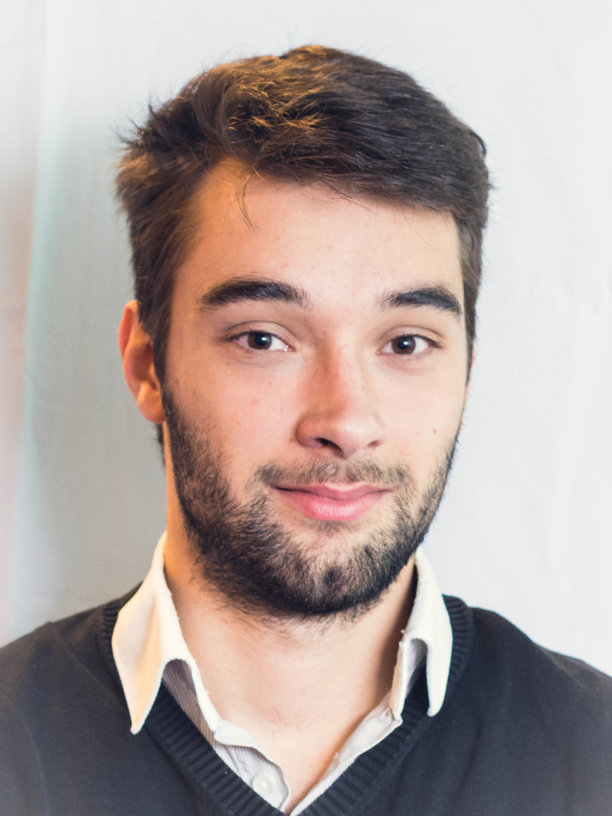
\includegraphics[scale=0.5]{picture}City}, grade, description
\cventry{2012 -- 2014}{DUT Informatique (Two-year core studies diploma in computer science)}{IUT de Nantes}{Nantes}{}{}

\section{Computer skills}
% \cvcomputer{category}{programs}{category}{programs}
% \cvdoubleitem{subtitle}{text}{subtitle}{text}
\cvitem{Programming languages}{Bash, C, Java (SE and EE), PHP, HTML, CSS, Javascript, Haskell (notions), Scala (notions)}
\cvitem{Modeling}{UML}
\cvitem{Databases}{Oracle, MySQL, PostgreSQL, Microsoft SQL Server (notions)}
\cvitem{Operating systems}{Windows XP/7/8, GNU/Linux (Debian)}
\cvitem{Tools}{Apache2, iptables, Fail2ban, OpenVPN, Git, Subversion}
%\cvitem{Software}{LaTeX, Microsoft Office, LibreOffice, Adobe Photoshop}

\section{Languages and other skills}
\cvlanguage{French}{Mother tongue}{}
\cvlanguage{English}{European B2 level (Independent User: Upper intermediate)}{\textbf{Toeic 895/990}}
\cvitem{Other}{Knowledge in communication and business management}

\section{Hobbies}
I love to discover new languages and to share my knowledge. I often attend computer sciences meetings (DevFest, Web2Day). I am a fervent defender of \textbf{free software} and \textbf{open source}.\\I've been playing the guitar for nine years. I workout with friends on my free time.
\end{document}
